% This is LLNCS.DEM the demonstration file of
% the LaTeX macro package from Springer-Verlag
% for Lecture Notes in Computer Science,
% version 2.4 for LaTeX2e as of 16. April 2010
%
\documentclass{llncs}
%
\usepackage{graphicx}
\usepackage{makeidx}  % allows for indexgeneration
\usepackage[T1]{fontenc}
\usepackage[utf8]{inputenc}
\usepackage{upquote}
%
\begin{document}
%
\frontmatter          % for the preliminaries
%
%\pagestyle{headings}  % switches on printing of running heads
%
%
\title{QVTs: A TGG-like graphical representation for efficient Declarative Model to Model Transformation scheduling.}
%
\titlerunning{QVTs - a TGG-like representation}  % abbreviated title (for running head)
%                                     also used for the TOC unless
%                                     \toctitle is used
%
\author{Edward D. Willink}
%
\authorrunning{Edward D. Willink} % abbreviated author list (for running head)
%
%%%% list of authors for the TOC (use if author list has to be modified)
\tocauthor{Edward Willink}
%
\institute{Willink Transformations Ltd., Reading, UK,\\
\email{ed \_at\_ willink.me.uk}
}

\maketitle              % typeset the title of the contribution

\begin{abstract}
Graph Grammars have been providing an increasingly sound foundation for Graph Transformation for nearly 50 years. 20 years ago, the enthusiasm surrounding the Model Driven Architecture motivated the OMG to start standardization of the QVT Model to Model transformation language. Sadly, the M2M work ignored the considerable overlap with GT and is much the worse for it. This paper shows how a graphical approach can resolve many of the M2M challenges and hopefully start to bridge the gap between the GT and M2M communities. 
\keywords{M2M, Model to Model Transformation, Graph Transformation, QVT, Scheduling, TGG}
\end{abstract}
%

\section{Introduction}

Within the academic community, the work on Single Push Out and Double Push Out established the principles of Graph Transformation~\cite{GT}. Triple Graph Grammars~\cite{TGG} leverage this foundation to provide a formulation that is more practical for model transformation. A TGG implementation is available via the Eclipse Henshin project~\cite{Eclipse-Henshin}.

Within the industrial community, the utility of models was recognized leading to the Object Management Group's Model Driven Architecture~\cite{MDA-1.0}. Model transformation was recognized as important and so the OMG requested proposals for a model Query/View/Transformation language. The eight initial submissions eventually merged into a triple language specification~\cite{QVT-1.0}; one imperative language, QVTo (Operational Mappings), and two declarative languages, QVTc (Core) and QVTr (Relations). Only QVTo has a flourishing implementation. QVTc was never implemented, despite the `c' suggesting it is a core that `o' and `r' extend. The two original QVTr implementations, ModelMorf and Medini QVT have remained proprietary and have not prospered. The Eclipse QVTd project~\cite{Eclipse-QVTd} has provided QVTc and QVTr editors for many years, but it is only relatively recently\footnote{As part of the Eclipse Neon release in June 2016.} that any execution functionality has been available.

Unfortunately the industrial community ignored the significant overlaps between QVTr and TGG. The lack of accurate or detailed QVTr publications has made it hard for the academic community to investigate the overlap in detail.

In this paper we outline the QVTs\footnote{QVTs is not part of the OMG specification} graphical representation that facilitates visualization of the Eclipse QVTd schedule synthesis. In Section~\ref{Background}, we introduce a running example and highlight characteristics of navigable opposites and declarative execution. The QVTs representation is described in Section~\ref{QVTs representation} and exploited in for static scheduling in Section~\ref{QVTs Exploitation}. Section~\ref{Related Work} presents related work and Section~\ref{Conclusion} concludes.

%\footnote{A Mapping is also known as a Relation or a Rule}

\section{Background}\label{Background}

\subsection{Running Example}

For most of the examples in this paper we will re-use \cite{Willink-ICMT2017} a very simple, but surprisingly troublesome, transformation that copies of a cyclic doubly linked list with reversed element order. The UML metamodel is shown in Fig~\ref{fig:Doubly Linked List UML Metamodel}. 

\begin{figure}[h]
	\centering
	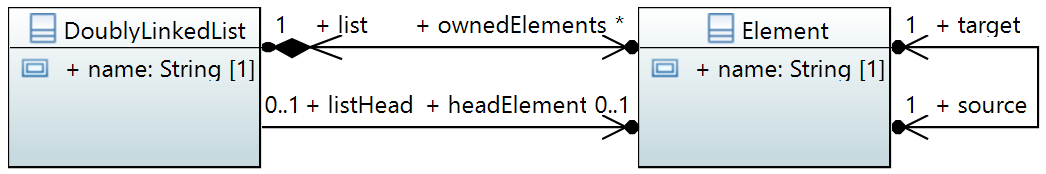
\includegraphics[width=0.95\textwidth]{doublylinkedlist.png}
	\caption{Doubly Linked List UML Metamodel.}
	\label{fig:Doubly Linked List UML Metamodel}
\end{figure}

There are just two classes, a \verb$DoublyLinkedList$ that has many \verb$Element$s, composed by the \verb$DoublyLinkedList::ownedElements$ relationship. A doubly-linked-list of \verb$Element$ is established by the \verb$Element::source$/\verb$Element::target$ bidirectional relationship. A particular \verb$Element$ is distinguished as the list head via the \verb$DoublyLinkedList::headElement$ relationship.

\subsection{Navigation and Opposites}

The Eclipse QVTd tooling leverages a little known capability of OCL; all associations are unconditionally navigable at analysis time. In UML, the role names on the ends of Associations distinguish alternate navigations from a common source. The arrows on the ends of Associations identify which ends are navigable at run-time. OCL is specified against the metamodel and so all role names are accessible in OCL. OCL provides mechanisms for defining and disambiguating omitted role names. As an extension of OCL, QVT can navigate a relationship such as \verb$DoublyLinkedList::headElement$ in either direction.

%run-time navigability of a relationship is denoted by the direction of an arrow on the line representing the relationship. A bidirectional relationship may be drawn with an arrow at each end. At run-time a navigable relationship will typically incur the cost of a slot in the source instance to point at the target end. A unidirectional relationship such as \verb$DoublyLinkedList::headElement$ therefore avoids incurring the cost of a to-$DoublyLinkedList$ slot in each \verb$Element$ but imposes a limitation that the navigation via the \verb$Element::listHead$ is not possible. %In this example, this is not much of a limitation since the \verb$Element::list$ relationship gives a similar result.

% A QVT transformation is analyzed at analysis time, therefore the unnavigable role-names such as \verb$Element::listHead$ are available for use by a QVT transformation and its tooling.

%Again in UML, the unnavigable opposite end of DoublyLinkedList::headElement may be given a role name such as "headList" in which case the corresponding unnavigable Property is owned by the Association rather than the Element class. This role name is available for use in OCL expressions. Even if the role name is missing, OCL provides rules for automatically synthesizing an unambiguous value; typically the target class Name. Thus the OCL navigation from anElement as anElement.DoublyLinkedList will navigate the DoublyLinkedList::headElement relationship in reverse returning a non-null DoublyLinkedList or null according to whether anElement is the headElement.

%When UML is converted to EMOF or Ecore, the Associations and Association-owned Properties are discarded. \verb$Element::listHead$ is not navigable in Ecore. However the importance of not discarding names used in OCL Constraints has led to MOF Tags or Ecore EAnnotations to preserve the required name. \verb$Element::listHead$ is navigable in an OCL expression exploiting a correctly serialized Ecore metamodel.

%In OCL, it not sufficient to evaluate \verb$anElement.listHead$ to determine the \verb$DoublyLinkedList$; we need to retain whether the value is optional, i.e. \verb$DoublyLinkedList[?]$, or a not-empty OrderedSet, i.e. \verb$DoublyLinkedList[+] \{ ordered, unique \}$. This information is also preserved as Ecore EAnnotations, but has yet to be standarized as MOF Tags.

%The importance of this will become clear when we navigate from a input model element to its trace in a QVTs mapping.

\subsection{Declarative Transformation Execution Schedule}

For a traditional functional/imperative/procedural program, a call tree specifies the order in which each stage of execution occurs. This should ensure that the inputs of each stage are provided by a previous stage. Unfortunately in complex programs, particularly those with global state or multiple threads, this does not always happen. The result provides for exciting debugging opportunities.

A declarative transformation eliminates these hazards by only specifying what must happen in each stage\footnote{a stage is variously a mapping, partition, relation or rule}. It is the responsibility of the execution engine to ensure that stages execute in an appropriate order. Naively, each stage may be attempted for arbitrary elements in an arbitrary order. If inputs are not available, the attempt must be aborted and retried later. Fig~\ref{fig:NaiveExecution} shows this.

\begin{figure}[h]
	\centering
	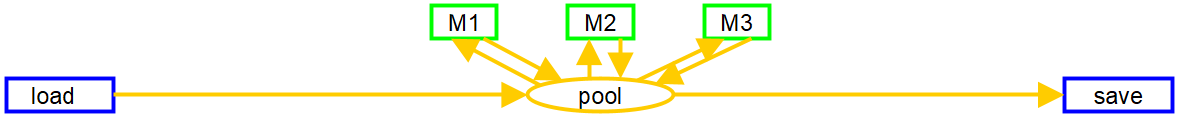
\includegraphics[width=0.95\textwidth]{NaiveExecution.png}
	\caption{Naive Declarative Transformation Execution.}
	\label{fig:NaiveExecution}
\end{figure}

A \verb$load$ stage loads all the input model elements into a \verb$pool$, from which attempted executions of the \verb$M1$, \verb$M2$, \verb$M3$ stages are repeated until execution completes. Then the \verb$save$ stage executes. The naive repetition of stages and permutation of input elements may easily lead to quadratic or worse execution performance. This performance is aggravated by the costs of keeping track of which inputs are ready, and which executions need a retry.

The strong typing of a declarative transformation provides ample opportunities for analysis so that we can hope to find an efficient schedule such as Fig~\ref{fig:SmartExecution}.

\begin{figure}[h]
	\centering
	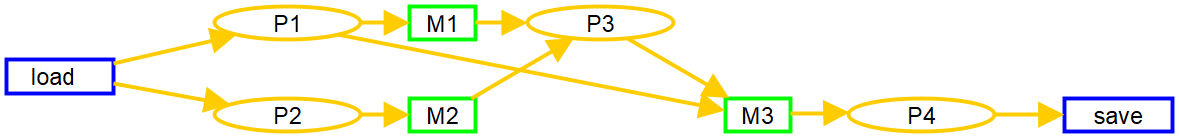
\includegraphics[width=0.95\textwidth]{SmartExecution.png}
	\caption{Smart Declarative Transformation Execution.}
	\label{fig:SmartExecution}
\end{figure}

The \verb$load$ now separates input elements into distinct \verb$P1$, \verb$P2$ pools whose element types suit the downstream \verb$M1$ and \verb$M2$ consumers. These produce to a distinct \verb$P3$ pool for \verb$M3$.

The smart schedule is a directed acyclic graph amenable to efficient scheduling. Given an accurate analysis, all \verb$M1$ and \verb$M2$ executions occur before any \verb$M3$; no time need be wasted attempting \verb$M3$ before \verb$M1$ and \verb$M2$ have completed. Consequently no time need be consumed testing whether \verb$M1$ and \verb$M2$ have completed.

Finding the smart schedule is the motivation for the QVTs representation described in this paper.

The need to find a smart schedule is particularly important for QVTr, since QVTr lacks the imperative workarounds that some declarative languages use to solve too-hard problems. For complex transformations, a first pass may create the output elements in a tree structure and then a second pass may elaborate the tree to form a more complex graph structure. Sequencing these passes requires the programmer to understand and use some limited imperative capabilities within the declarative transformation language. QVTr is more powerful; the programmer is not required to understand the practicalities of the execution schedule, rather the QVTr analysis or run-time must solve the problem.

\subsection{Eclipse QVTd Tool Chain}

A simple tool using a naive execution schedule could attempt an interpreted execution using little more than a transformation language loader and interpreter. Eclipse QVTd provides an efficient execution using the tool chain shown in Fig~\ref{fig:QVThorizontalAlphabet}.

\begin{figure}[h]
	\centering
	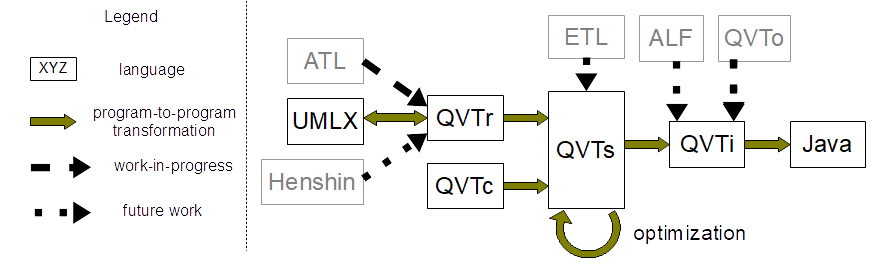
\includegraphics[width=0.95\textwidth]{QVThorizontalAlphabet.png}
	\caption{QVTd Tool Chain.}
	\label{fig:QVThorizontalAlphabet}
\end{figure}

The QVTr language support is followed by a transformation to the QVTs graphical representation. After optimization this is converted to an assembler-like QVTi imperative representation. This can be executed directly by an interpreter or code generated using an extension of the Eclipse OCL Java code generator to give pure Java code. The tool chain is open for re-use by other languages. UMLX~\cite{UMLX} is fully supported, ATL~\cite{Eclipse-ATL} partially.

%(It was originally planned to follow the OMG specification exposition of transforming QVTr to QVTc as part of a progressive transformation via unidirectional QVTu and minimal QVTm representations. However work on the semantics of  overriding relations, which have no QVTc counterpart required too many time consuming idiomatic adjustments to QVTc, QVTu and QVTm to support a language research activity. The increasing utility of the QVTs representation motivated a rewrite so that QVTr now transforms directly to QVTs. QVTc continues to use the intermediates.)


\section{The QVTs representation}\label{QVTs representation}

In this paper we elaborate the auto-generated QVTs graphical representation and its many similarities to TGG. The most obvious similarities between TGG rules and QVTs mappings are:

\begin{itemize}
\item diagrams based on UML Object Diagrams 
\item patterns with nodes for Class-typed variables, edges for typed-relationships
\item three swim lanes: left : correspondence(TGG), middle/trace(QVT) : right
\item metamodel typing for all three lanes, with accurate multiplicities
\item no deletion
\item green coloring for additions (also ++ annotation for TGG)
\item positive Constraints, rather than Negative Application Conditions
\end{itemize}

The main practical difference is that TGG Rules are manually created programming artefacts, whereas QVTs mappings are auto-generated visualizations\footnote{the content is auto-generated, the aesthetic layout is currently manual} derived from QVTr Relations. 

The most fundamental difference is in the use of OCL. A TGG Assignment or Constraint node has an opaque embedding of an OCL expression. QVTs has nodes for the variables, and edges for the navigation, of an OCL expression AST. QVTs reifies an Attribute as a DataType-typed node and a Property-typed edge.

Other differences are:

\begin{itemize}
\item TGG has a shortform for endogenous (often in-place) transformations
\item QVTs resolves in-place\footnote{in-place support is future work} by a post-synthesis optimization / synchronization
\item TGG rules can be un-directional, QVTs mappings are for a chosen direction
\item A negative link in TGG is a (positive) link to a \verb$null$ constant in QVTs
\item QVTr auto-generates the middle metamodel with accurate opposites
\end{itemize}

Since the QVTs is auto-generated, a variety of rendering capabilities can be used to provide an enhanced visualization.

\begin{itemize}
%\item QVTs visualizes arbitrary OCL, including Positive Predicates, graphically
\item QVTs uses multiple colors to show lifecycle
\item QVTs arrows show to-one(-or-zero) navigability
\item QVTs line styles show nullability and distinguish matches/expressions
%\item QVTs exploits OCL's opposite navigation
\end{itemize}

\subsection{QVTs Synthesis - QVTr to QVTs conversion}\label{QVTs Synthesis}

Space limitations permit only the observation that the conversion from QVTr to QVTs normalizes QVTr high level facilities and syntax sugar to a simpler form.

\begin{itemize}
	\item Inherited Class matching
	\item Inherited Property matching
	\item Relation Overriding
	\item Exogeneous and Endogeneous Transformations
	\item Top and Non-Top Relations
	\item Keys
	\item Trace Metamodel Synthesis
\end{itemize}

\subsection{Trimmed list2list Mapping}

The two mappings for our example are shown in Fig~\ref{fig:list2list Mapping} and Fig~\ref{fig:element2element Mapping}. The \verb$list2list$ mapping is the TGG-Axiom. It is simplified in Fig~\ref{fig:Trimmed list2list Mapping} to ease discussion.

\begin{figure}[h]
	\centering
	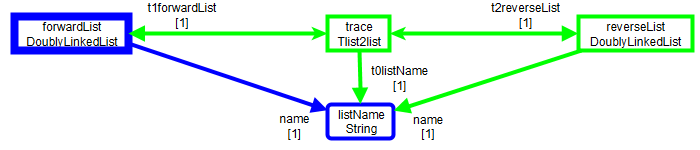
\includegraphics[width=0.95\textwidth]{list2listTrimmed.png}
	\caption{Trimmed list2list Mapping.}
	\label{fig:Trimmed list2list Mapping}
\end{figure}

The three columns and top row are essentially identical to TGG. On the left an input pattern variable named \verb$forwardList$ of type \verb$DoublyLinkedList$ is transformed, via a middle variable named \verb$trace$ of type \verb$TList2List$, to an output pattern variable named \verb$reverseList$ of type \verb$DoublyLinkedList$.

The green coloring identifies elements created by the mapping in similar way to green coloring and ++ annotations in TGG. The blue coloring identifies elements that are present in the input model.

The labels and multiplicities on the arrows show the role names and multiplicities of the relationships in the metamodels.

QVTs arrows are different to UML and TGG. A QVTs arrow head identifies a direction in which the navigation yields precisely zero or one element. A triangular arrow as from \verb$trace$ to \verb$forwardList$ identifies a direction that is available at run-time. The curved arrow as from \verb$forwardList$ to \verb$trace$ identifies an opposite navigation that, if used, may require additional run-time support.

Below the top row, we have an additional DataType-typed variable named \verb$listName$ and of type \verb$String$. It is an Attribute. It is drawn as a rounded rectangle to distinguish it from a Class-typed rectangle. DataTypes exist by value, rather than as objects and so may be shared/duplicated at the convenience of the implementation. We therefore draw navigation arrows from each of the objects for which \verb$listName$ is their name; there is no need for a separate constraint node such as \verb$reverseList.name = forwardList.name$. Navigation from a DataType-typed node is of course impossible.

\subsection{Full list2list Mapping}

The full mapping for \verb$list2list$ is shown in Fig~\ref{fig:list2list Mapping}.

\begin{figure}[h]
	\centering
	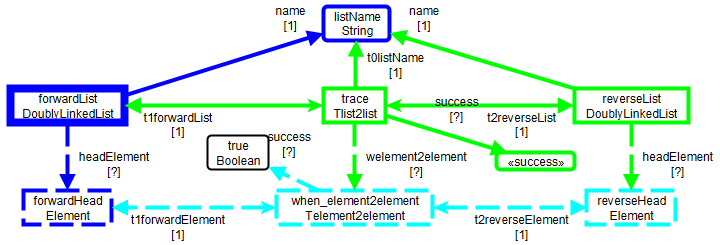
\includegraphics[width=0.95\textwidth]{list2list.png}
	\caption{Full list2list Mapping.}
	\label{fig:list2list Mapping}
\end{figure}

The additional bottom row transforms the \verb$forwardList.headElement$ to the \verb$reverseList.headElement$. The \verb$headElement$ is optional, and so may be \verb$null$. This is denoted by the \verb$[?]$ multiplicities, dashed edges and borders. Execution of a mapping requires solid nodes and edges to match; dashed nodes and edges are ignored for matching purposes, but are used by additional predicates and result computations.

Assignment of \verb$reverseList.headElement$ is not possible until \verb$reverseHead$ Element has been created by the \verb$element2element$ mapping whose execution is reified by the \verb$when_element2element$ variable of type \verb$TElement2Element$. The cyan coloring identifies nodes and edges that must be available from somewhere else before this mapping can execute.

The full mapping also shows the bookkeeping \verb$success$ variable. The green arrow to the green \verb$«success»$ node causes a \verb$true$ or \verb$false$ value to be assigned to \verb$trace.success$ according to the successful execution of the mapping. \verb$«success»$ is unusual in that it is the only green element that it is assigned in the case of a failure. This enables other mappings to react to the success or failure. This can be seen in the \verb$when_element2element.success$ cyan navigation to the \verb$true$ black compile-time constant; the \verb$list2list$ mapping fails if the \verb$when_element2element$ fails.

\subsection{Full element2element Mapping}

The full mapping for \verb$element2element$ is shown in Fig~\ref{fig:element2element Mapping}.

\begin{figure}[h]
	\centering
	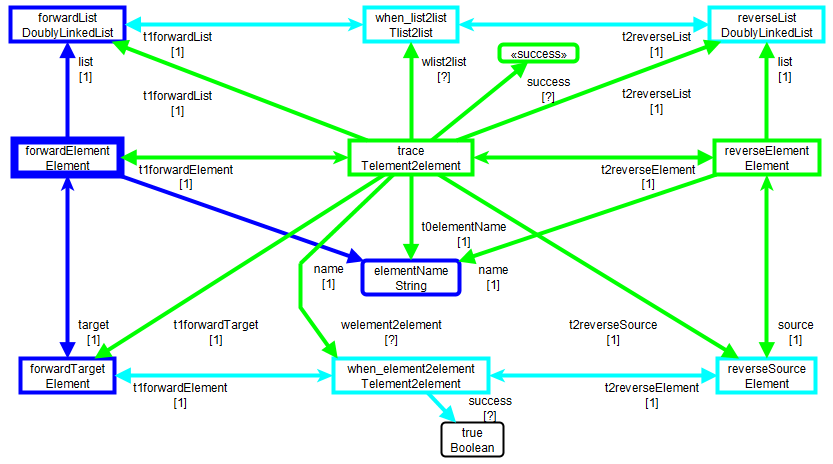
\includegraphics[width=0.95\textwidth]{element2element.png}
	\caption{element2element Mapping.}
	\label{fig:element2element Mapping}
\end{figure}

It is structurally very similar to \verb$list2list$. \verb$forwardElement$ is copied to \verb$reverseElement$ via a \verb$trace$ element of type \verb$TElement2Element$. Copies of the \verb$forwardElement.list$ and  \verb$forwardElement.target$ elements are assigned to \verb$reverseElement.list$ and \verb$reverseElement.source$. In each case, the cyan copy created elsewhere is located by an opposite navigation from the blue source to its cyan trace and then by forward navigation to the cyan copy. Only the success of \verb$when_element2element$ needs checking since \verb$list2list$ has no independent failure mechanism. Note that since \verb$DoublyLinkedList::ownedElements$ is a one-to-many relationship, it is not shown on the diagram. A unique set of object matches is available by traversal from the \verb$forwardElement$. There is no such similar unique set available from the \verb$forwardList$.

\subsection{Local Mapping Analysis}

The line styles and colors show the results of some minor analyses.

\subsubsection{Heads Analysis}The result of the more significant heads analysis is shown by the thick border of \verb$forwardList$ in Fig~\ref{fig:list2list Mapping} and \verb$forwardElement$ in Fig~\ref{fig:element2element Mapping}. The set of heads of each mapping is the smallest set of non-green nodes from which all nodes can be reached by traversing to-one(-or-zero) relationships. For nearly all mappings, just like the examples, a set of one node is sufficient.

A single head provides the start of a one-dimensional matching search strategy; for each \verb$Element$ model element we must attempt the \verb$element2element$ mapping. The full pattern match can be found in constant time following the to-one(-or-zero) relationships. This is clearly much more efficient than a super-naive attempt at a seven-dimensional permutation of all possible model elements against the seven blue and cyan nodes in \verb$element2element$.

The diagram therefore shows that we can navigate from the \verb$forwardElement$ to precisely one \verb$trace$ using an inferior navigation path and from there to precisely one \verb$reverseElement$ using a good navigation path. %No arrow is shown for \verb$forwardList.ownedElements$ since this is a one-to-many relationship. The \verb$forwardElement$ can navigate to precisely one \verb$forwardList$, but the converse yields many \verb$forwardElement$s.

%The ability to locate a pattern of objects in precisely to-one relationship is very important. The \verb$forwardList$ is therefore drawn with a thicker boundary to distinguish its status as a head, from which everything else can be reached.

%We have already seen the head analysis; identification of an input node from which all other nodes can be reached by unambiguous to-zero-or-one navigation. This analysis usually yields a single head, but not always. Some mappings exploit two or even three independent input elements as part of their processing. This is undesirable, since the execution must consider the Cartesian product of the available inputs probably leading to quadratic or cubic execution time. But if that is what is needed that is what must be done. A mapping may therefore have multiple heads.

\subsubsection{Producer/Consumer Analysis}The green coloring clearly identifies nodes and edges that are created/produced by the mapping execution. Similarly blue and cyan coloring identifies nodes and edges that are consumed. The blue elements come from the input model and are therefore available just as soon as the input model loading completes. The cyan elements are more troublesome; they come form somewhere else. This gives the simple  scheduling policy that consumed cyan elements must be computed before green elements can be produced.

The \verb$list2list$ mapping produces 2 Class-typed nodes, 1 DataType-typed node and 7 edges (green). It consumes 2 Class-typed nodes and 3 edges (cyan).

Looking at \verb$list2list$ we see that there is a green \verb$TList2List$ and a cyan \verb$TElement2Element$, therefore \verb$list2list$ cannot execute until the appropriate \verb$element2element$ has executed. Similarly \verb$element2element$ has a green \verb$TElement2Element$ and a cyan \verb$TList2List$, therefore \verb$element2element$ cannot execute until the appropriate \verb$list2list$ has executed. At compile-time, without knowledge of the appropriate instance, the static schedule must wait for all instances. There is a cyclic dependency; a deadlock.

\subsubsection{Partitioning}The \verb$list2list$ / \verb$element2element$ deadlock is easily broken by using multiple passes. A first pass creates the new \verb$DoublyLinkedList$ and \verb$Element$ elements, a second pass assigns the \verb$DoublyLinkedList.headElement$. We can minimize the likelihood of deadlocks by partitioning each mapping into atomic micromappings with a single green element per micromapping. This proves to be excessive and so we partition into a number of partitions each tackling a separate `theme':

\begin{itemize}
	\item activator: to create the green trace element and green edges to input elements
	\item local: predicate to verify that cyan elements are locally satisfied
	\item global: predicate to verify that cyan elements are globally satisfied
	\item speculated: to create the green output node(s) and assign trace success
	\item per-edge: for each remaining green edge to a green output node 
\end{itemize}

%Generically, the problem is that QVTr does not require the mappings to be broken up into implementable passes.

%If our doubly-linked-list was a daisy-chain we can break the metamodel cycle by considering the model elements, starting at the null-source end and iterating along the list.

%But our list has a non-null source so it must be a cycle in the model as well; we have a deadlock.

\subsubsection{OCL Expression Analysis}
	
The list example is too simple to demonstrate the use of OCL within QVTs. We therefore use a mapping from the Families2Persons example to show OCL expressions in Fig~\ref{fig:Simple Expressions Example}.

\begin{figure}[h]
	\centering
	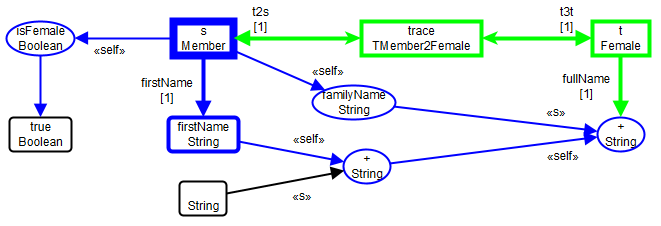
\includegraphics[width=0.95\textwidth]{SimpleExpressionExample.png}
	\caption{Simple Expressions Example.}
	\label{fig:Simple Expressions Example}
\end{figure}

The matched part of the mapping is shown by the creation of two green \verb$trace$ and \verb$t$ nodes from the blue \verb$s$ node.

At the left an operation call to the \verb$isFemale$ query using \verb$s$ as its \verb$«self»$ input is shown using an ellipse. The output is consumed by the \verb$true$ constant. The overall truth of the mapping is only satisfied when everything is true, therefore if \verb$isFemale$ returns false the match fails. The graphics shows the constraint \verb$s.isFemale() = true$.

In the lower part of the figure we see the string concatenation for the assignment \verb$t.fullName = s.firstName + ' ' + s.familyName()$.

OperationNodes and ArgumentEdges are shown with thin line-styles. Black coloring is used for compile time constants. Blue coloring is used for computations that can be made as soon as the input model is loaded. Only the actual assignment edge for \verb$t.fullName = ...$ is green. The ArgumentEdges are annotated with the receiving parameter name such as \verb$«self»$ to eliminate ambiguity. These nodes and edges are really just a visualization of the OCL AST. The part of the ATL2QVTr transformation shown in Fig~\ref{fig:Complex Expressions Example} has many more complex usages.

\begin{figure}[h]
	\centering
	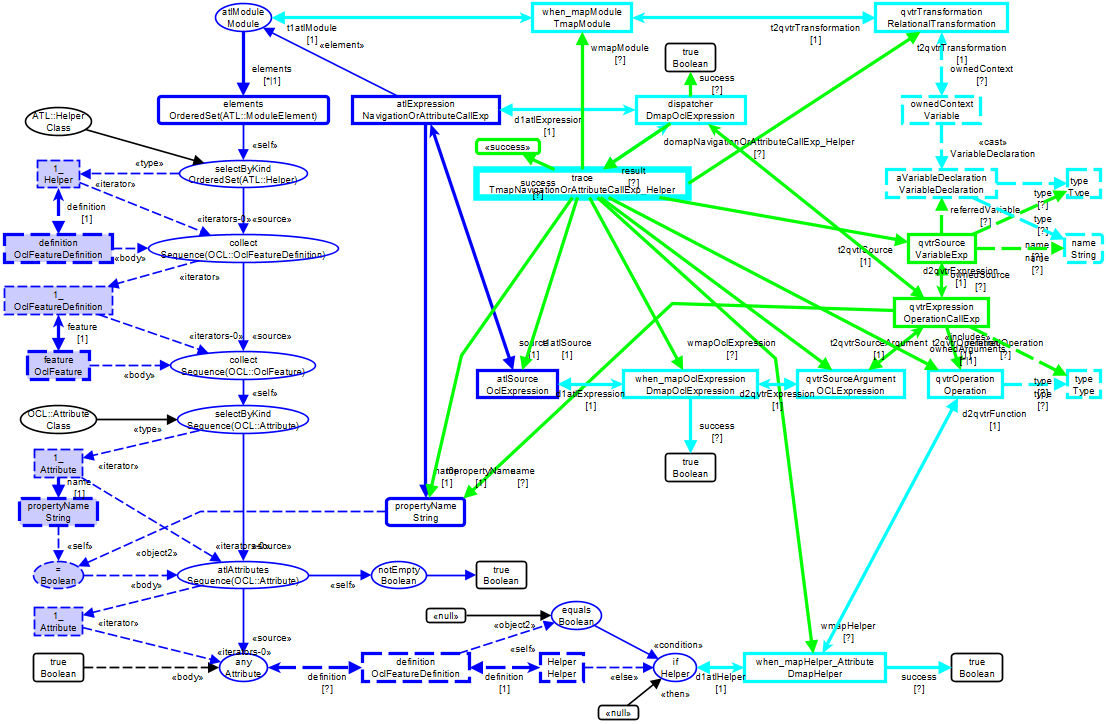
\includegraphics[width=0.95\textwidth]{ComplexExpressionExample.png}
	\caption{Complex Expressions Example.}
	\label{fig:Complex Expressions Example}
\end{figure}

The upper part of the left hand two columns evaluate
\begin{verbatim}
atlAttributes = atlModule.elements
  ->selectByKind(atlMM::Helper)._definition.feature
  ->selectByKind(atloclMM::Attribute)->select(name=propertyName)
\end{verbatim}
This demonstrates the use of DataType-typed Collection nodes and IteratorNode variables in body expressions. It also demonstrates that node sharing in the graphical representation corresponds to Common Subexpression Elimination in traditional tooling.

\subsection{Operation Analysis}

OCL expressions may call operations, which may involve navigations and consequently an operation may fail if its execution is premature. Operations have no mechanism for aborting and retrying later and so it is the callers responsibility to anticipate the navigations and guarantee that the execution is not premature. This guarantee requires a deep analysis of each operation call. Additional consumer dependencies capture the analysis result.

A straightforward analysis of the potential dependencies of each OCL navigation must take a very pessimistic view of the dependencies for utility functions whose argument types are high up polymorphic inheritance trees. These pessimistic dependencies can lead to unnecessary dependency cycles. A more precise analysis specializing each OCL call expression to the known calling types can avoid these cycles.

%The scheduling algorithms rely on a global dependency analysis which must be accurate to avoid malfunctions due bad schedules not ensuring required inputs are available. Absolute precision is impossible but we can avoid malfunction by providing a pessimistic analysis where analysis is too hard. However too much pessimism and everything depends on everything making an efficient static schedule infeasible. We need a very narrow pessimism.

%Almost arbitrary OCL expressions can be used as guards and initializations within a mapping. These expressions may therefore contain calls to operations that may involve accesses to properties potentially within iterations or nested operations. These property accesses must be satisfied before the mapping invoking an operation can execute. Many operations have rather general arguments such as a NamedElement leading to rather general dependencies. However at the invocation we may know that the argument can only be a Package enabling an operation analysis to be specialized for its known argument types giving significantly narrower dependencies.

\section{QVTs Exploitation - Static Scheduling}\label{QVTs Exploitation}

The QVTs representation analysis supports derivation of an efficient schedule.

\subsection{Global Analysis}

The cyan consumer analysis identifies which nodes and edges are consumed by each partition. These can be joined to the corresponding green producers by a pool for the type of each node or edge as shown in Fig~\ref{fig:SmartExecution}. Additionally the heads analysis identifies which consumers require the corresponding node to be passed-by-value. All other consumptions can be computed by navigation from a head. We therefore refer to these additional consumptions as passed-by-existence.

%The local analysis with its cyan/green colouring identifies where each typed-nodes and edges is produced or consumed. We can use this to provide a global analysis whose nodes are producing/consuming mappings and the typed-node/edge elements that are produced/consumed. The directed edges of the global analysis graph show the data flow from producer to typed-element and from typed-element to consumer. This analysis directly corresponds to a plausible run-time model in which a mapping is invoked to consume an element from a pool of consistently-typed available elements and produce an element to another pool of consistently-typed elements. Mappings are invoked when input pools have elements to be consumed.

The global consumer/producer analysis for our simple two mapping example is shown in Fig~\ref{fig:RawSchedule}.

\begin{figure}[h]
	\centering
	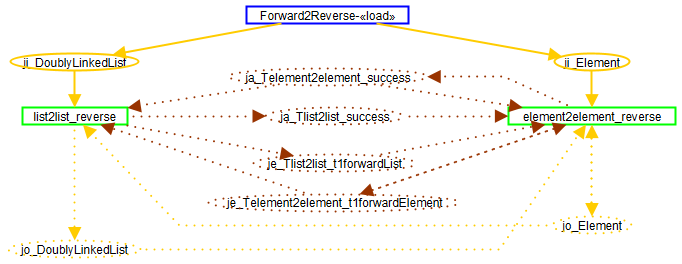
\includegraphics[width=0.95\textwidth]{RawSchedule.png}
	\caption{Raw Producer/Consumer Dependency Graph.}
	\label{fig:RawSchedule}
\end{figure}

The blue mapping at the top is the auto-generated loader responsible for loading the input model and distributing the relevant model elements to suitable pools.

The two orange ellipses are the input pools, one for the \verb$DoublyLinkedList$ element and the other for the \verb$Element$ elements. The incoming arrows show that the elements are produced by the loader.

The two green rectangles are the two unidirectional mappings\footnote{the $reverse$ suffix denotes the chosen direction of QVTr execution} each consume a \verb$DoublyLinkedList$ or \verb$Element$ element via a solid incoming orange arrow.

In addition to consuming model element node instances from the input model, each mapping execution also consumes edge instances. The pools of consumed/produced edges are shown using brown ellipses. The top brown ellipse shows that the \verb$Telement2element::success$ property is produced by the \verb$element2element$ mapping and consumed by both mappings.

The \verb$list2list$ mapping has four incoming arrows indicating that an element must be available in each of four source pools to support a successful execution. The solid arrow passes the \verb$DoublyLinkedList$ element by value. The remaining arrows are dotted to indicate pass-by-existence. 


%This does not however mean that the mapping implementation requires four inputs, and certainly does not require a four-dimensional permutation of all possible inputs. Our local analysis has identified that once we have the value for the head element, we can locate all the other elements by navigation from the head. The head element is made available on the solid orange arrow from the DoublyLinkedList pool. The remaining elements are computable provided the required elements are present in four pools linked by incoming dotted arrows. The solid arrow therefore indicates a traditional pass-by- value, whereas a dotted arrow indicates a virtual pass-by-existence. A pool that is only consumed by dotted arrows is also shown dotted; it is a virtual pool that is never used in a correct scheduled implementation. This is particularly convenient for edges that have no traditional mechanism for passing.

The diagram shows many cycles between the two mappings. An efficient purely static schedule is not possible.

\subsection{Partitioned Schedule}

%One of the problems is that QVTr allows the multiple passes needed by a successful execution to be folded into a single exposition, requiring that list2list be fully executed before element2element and vice-versa.

%We could just reject the program and provide the programmer with some guidelines on how to write more acceptable transformations. Or we can solve the problem, by partitioning the mappings into much smaller micromappings that avoid spurious interdependencies. In the extreme, we could have a separate micromapping for each green node or edge to avoid any possibility that one green element interferes with another. However many of the green edges can be added automatically as soon as a green node is added and so a more pragmatic partitioning involves

%\begin{itemize}
%	\item activator: to create the green trace element and green edges to input elements
%	\item local: predicate to verify that locally determined cyan elements are satisfied
%	\item global: predicate to verify that globally determined cyan elements are satisfied
%	\item speculated: to create the green output node(s) and assign trace success
%	\item edge (multiple): for each remaining green edge to a green output node 
%\end{itemize}

Fig~\ref{fig:PartitionedSchedule} shows the more complex dependency graph that results after partitioning. The graph is topologically similar to Fig~\ref{fig:RawSchedule} with the partitioned \verb$list2list$ mapping replaced by 5 partitions on the left hand side and the partitioned \verb$element2element$ mapping replaced by 6 partitions on the right hand side.

\begin{figure}[h]
	\centering
	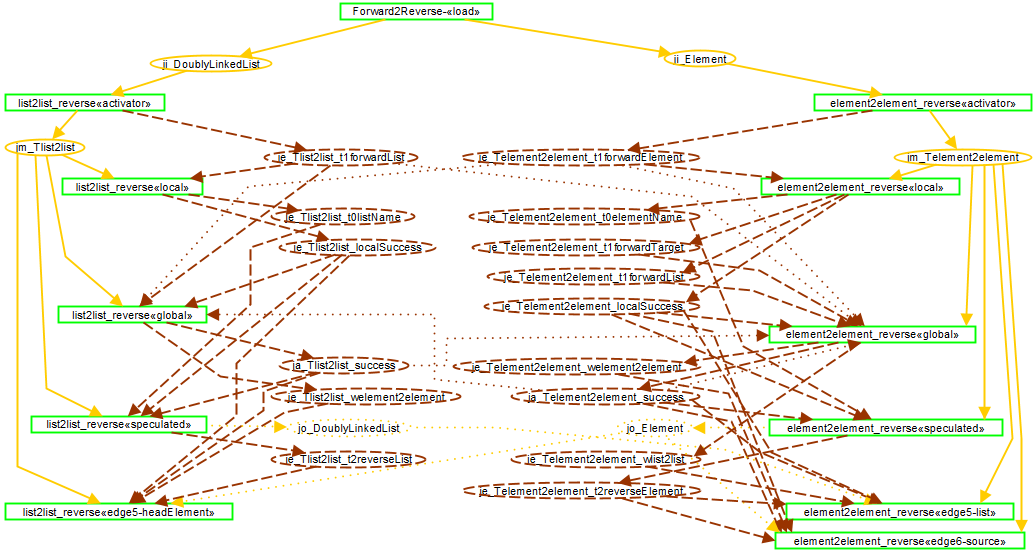
\includegraphics[width=0.95\textwidth]{PartitionedSchedule.png}
	\caption{Partitioned Producer/Consumer Dependency Graph.}
	\label{fig:PartitionedSchedule}
\end{figure}

At the top we see the activators have consumed their input model element and produced a corresponding trace element which is consumed by the local and other partitions.

At the bottom we see the speculated and edge partitions with inputs, outputs and no problematic cycles. Introducing a separate partition, that can be performed once everything else is ready, has resolved the cycle involving the assignment of \verb$DoublyLinkedList::headElement$.

Many of the dependencies use a dashed style. This is a much stronger version of pass-by-existence. The value is guaranteed to exist, the consumer can therefore use it without checking. In contrast the dotted line only indicates that the value may-be available; the consumer must test for readiness and arrange to retry until the required value is ready. Dashed lines are therefore efficient at run-time. Dotted lines incur run-time overheads for retries. For both dotted and dashed pools, no value is actually passed and so there is no need to provide run-time support; it is a virtual pool. It is the consumer that computes the passed-by-existence value and must check whether the computed value is ready.

\subsection{Speculation}

Further examination of Fig~\ref{fig:PartitionedSchedule} shows that we still have a cycle involving the global partitions and the success pools. This is because the cyclic list in this simple example is really troublesome; the transformation can only proceed if the mapping executions for each list element collaborate. When acyclic structures such as composition trees are involved, collaboration can be guaranteed. For genuinely cyclic structures a global mediator must be invoked at run-time.

%The problem is perhaps more easily seen in human terms. If I promise to show you my paper if you show me yours, we have three outcomes.

%\begin{itemize}
%	\item trust - two shows - we each show each other our papers
%	\item distrust - no shows - we do not show each other our papers
%	\item cheat - one show - one of us shows, the other doesn't
%\end{itemize}

%In the real world, cheating can be eliminated by a mediator who receives the promises to show then enforces the show. In the transformation world we have two consistent outcomes. Trust in which each element trusts that the neighbouring source element will be available to allow the rotation. Distrust in which each element cannot guarantee that the neighbouring source element is available and the transformation fails. Both outcomes are consistent with the transformation definition, although one produces a 'useful' output and the other does very little.

%Returning to the human example, it could be that I am superstitious and never trust anybody on Friday the 13th. Without a mediator this will lead to me cheating. With a mediator, you are just disappointed that I didn't show you my paper.

%In the transformation world, additional predicates may similarly make unconditional global trust unfounded. The local partition determines as much as possible speculatively before validating that speculation globally. The global partition performs an AND of the speculations to determine whether every participant is collaborating. The residual loop has therefore been reduced to the multiple contributions to an AND gate. 

\subsection{Cycle Elimination}

The dependency graph is only mostly acyclic, so we need a solution for the cyclic parts. This proves to be rather simple. Cycles are easily identified as the intersections of transitive predecessors and successors. Each cycle can be wrapped up rather like a Russian doll. The result is acyclic with respect to the dependency edges; cycles are localized to the Russian doll node that may have a further acyclic dependency graph inside. 

\subsection{Pass Allocation}

The acyclic directed dependency graph provides an ordering of the partitions so that we may allocate the partitions to sequential passes. Typically pass 0 for the loader, pass 1 for the activators, pass 2 for ... 
One or more pass numbers are allocated to each pool in accordance with the pass numbers in which each producer may add content.

These pass numbers are shown in the the Fig~\ref{fig:FinalSchedule} which also shows the results of some optimizations.

\begin{figure}[h]
	\centering
	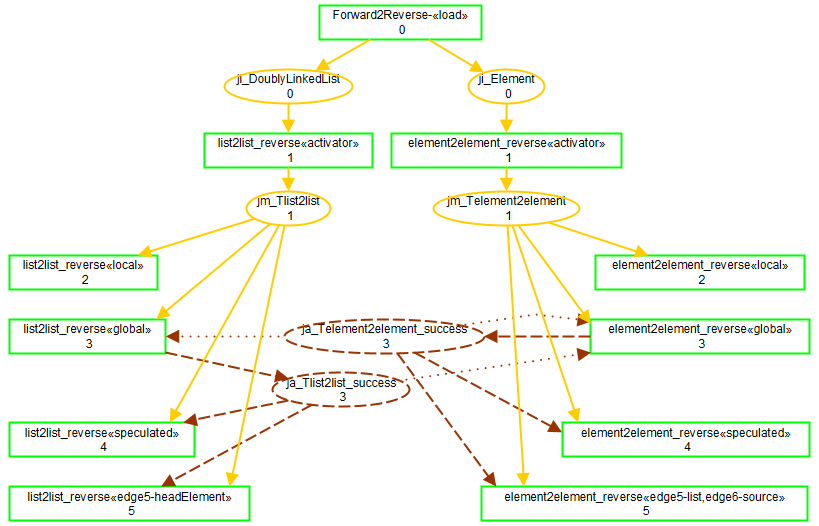
\includegraphics[width=0.95\textwidth]{FinalSchedule.png}
	\caption{Final Producer/Consumer Dependency Graph/Schedule.}
	\label{fig:FinalSchedule}
\end{figure}

%The figure also shows the results of some optimizations.

Virtual pools whose pass numbers are smaller than all the pass numbers of all their consumers are inherently safe and are removed. Only pass 3 involving the global speculation remains indicating a need for run-time support.

Sibling partitions sharing the same failure mechanisms are merged.

%(Further merging is a future work opportunity.)

%Overall we see that the \verb$DoublyLinkedLIst::headElement$ cycle has been eliminated by partitioning.

We also see that the solid orange arrows provide a very simple call-tree in which each partition has a single input avoiding the need for any complex multi-dimensional dispatch. The partitions for each pass can be concurrently executed one pass at a time, with the exception of pass 3 that requires a global mediation to resolve its instance cycle.

%The OMG specification defines the textual Concrete Syntax of QVTr using a grammar, an underlying Abstract Syntax model and indications as to how the two correspond. QVTr extends OCL and so its AS comprises a variety of OCL and QVT model elements. OCL encapsulates all access to a navigation edge as a PropertyCallExp or OppositePropertyCallExp\footnote{The OCL AS is not serializable without an OppositePropertyCallExp} to which QVT adds a PropertyTemplateItem. We therefore have three AS classes for a similar navigation concept. The conversion to QVTs normalizes these three as NavigationEdges. Similarly OCL's introduce let-variables, iterator-variables, context-varaible, and parameter-variables are augmented by shared-variables and pattern-variables in QVT. These are unified as PatternVariableNode and IteratorNode in QVTs.

%\subsubsection{Model Element Inheritance}

%Metamodels define classes that may generalize/extend/inherit-from/derive-from other classes. Consequently a mapping that consumes an instance of type B, may also consume an instance of any class that extends B. The global analysis to associate consumers to producers must therefore consider all possible super-productions. (The converse approach of considering all possible sub-consumptions may fail if the input model involves model elements from an extended metamodel.)

%Metamodels also define properties for classes which are inherited by derived classes. When considering production and consumption of, for instance, the NamedElement::name inherited by a Package or Class as a NamedElement::name is too pessimistic, since consumption of any name requires all names to have been produced. If instead we retain the precision that a Package::name is consumed, we can avoid requiring the producers of Class::name to have completed. Obviously a mapping that consumes NamedElement::name must wait for all names.


%\subsubsection{Relation Overriding}

%In many conventional languages operation polymorphic operation overloading is realized by a simple dynamic dispatch on the source type; the correct implementation is fully determined by the source type. 

%Overriding relations are more complex, since while the source type might uniquely select an override, guard conditions may cause the match to fail requiring an overridden relation to be attempted. There may be many same-typed relations distinguished by their guard conditions.

%QVTr supports the override of one relation by another, but neglects to specify the semantics. This is therefore a language design issue to be researched by vendors.

%Eclipse QVTr requires the root variables of an overriding relation to conform to those of an overridden relation and introduces an abstract relation to provide a flexible root of a family of overrides. At run-time all overrides are eligible for execution, but successful execution of an overriding relation causes the execution the overridden relations to fail. 

%The foregoing semantics can be realized in the QVTr to QVTs synthesis avoiding the need for special QVTs support. We require two levels of tracing, one for the overall polymorphic execution, and another for each participating attempt. Communication between the attempts uses the initially-null, eventually true/false success status of each trace.

%Execution of the polymorphic override proceeds in three phases with an initial activator and final verdict mapping for the overall family.

%\begin{itemize}
%	\item invocation activates each of the possible overrides and verdict with a null success status
%	\item once ready possible overrides attempt to execute assigning true/false success status, a successful execution also assigns overall success
%	\item once, and if, all possible overrides have a failed status, the verdict mapping assigns an overall failure  
%\end{itemize} 

%The eager activation of all possible overrides above is inefficient. Deferring activation of an overridden relation to %the failing override is a future optimization.   

%\subsubsection{Exogeneous and Endoogeneous Transformations}

%Exogeneous model to model transformations operate between models conforming to distinct metamodels. However for homogeneous transformations such as in-place transformations, input and output metamodels may be the same. This leads to considerable confusion if a too-simple type-based analysis is performed. When the same type can be both an input and output, everything ends up dependent on everything and an efficient static schedule is impractical.

%Eclipse QVTr avoids the problem of endogenous ambiguity by using a a datum-based rather than type-based analysis. A datum is a tuple of type and input/output domain. Analysis of an endogenous transformation is then no different to that of a exogeneous transformation.

%\subsubsection{Top and non-top Relations}

%QVTr provides two kinds of relation.

%Top relations are matched wherever a suitable pattern of input model elements can be found. Top relations are not invoked explicitly.

%Non-top relations are invoked explicitly within the context of a match found by another relation. When used extensively, non-top relations provide the programmer with the option to specify the matching schedule explicitly.

%Two distinct forms of invocation add implementation complexity. The Eclipse QVTr synthesis removes the distinction by creating an explicit call for each top level relation in the context of each matching input model element.

%\subsubsection{Trace Metamodel}

%The QVT specification is vague about the origins of the trace metamodel. It provides rules that suggest how a trace model can be synthesized, but these rules ignore consideration of collections, multiplicities and opposites. They also ignore the need for inter-relation communication to resolve overriding.

%Eclipse QVTr synthesizes a metamodel that resolves these problems and also annotates each trace property with its domain so that endogenous ambiguities are avoided.

\section{Related Work}\label{Related Work}

A catalog of optimizations has been proposed \cite{TGG-Optimization} for Triple Graphs; domain driven applicability, caching/indexing, static analysis, incremental execution. Many of these come for free in the current work.

Many papers refer to QVT, but few provide insight because the only exposition of QVT is its flawed specification. Too many authors have tended to regard an OMG specification as the work of the gods, whereas in practice a specification is the best endeavors of a small, sometimes very small, team of busy, underfunded, not always omniscient, contributors. Revised specifications are necessary to remedy defects as well as accommodate unforeseen use cases. The QVT specification is unique. It is the first time the OMG has standardized research work; it really should have started at version 0.0 to emphasize this.

The QVTr language is `formalized' by RelToCore, a hard to read transformation written in QVTr from QVTr to QVTc. QVTc is `formalized' using semi-formal language. Unfortunately the QVTc semi-formalization is incomplete and RelToCore neglects important concepts such as Collection matches and Relation overriding. RelToCore comprises over 1000 lines of the new QVTr language. RelToCore was written without the aid of language support tooling. It is therefore not surprising that when Eclipse QVTd started to provide QVTr editors, many syntactic and semantic problems were uncovered. Clearly the 1000 lines of QVTr that formalize QVTr have never been exercised.

Authors such as Stevens~\cite{Stevens-game} have endeavored to understand RelToCore and the QVTc semi-formalization and concluded that QVTr and QVTc are inconsistent despite QVTr being just a transformation away from QVTc. Westfechtel~\cite{Westfechtel} has endeavored to provide a bidirectional implementation of Families-to-Person and found that QVTr's check-mode\footnote{a check-mode execution precedes an enforce-mode to avoid the cost of an enforce} semantics are inconsistent with enforce-mode. This mandated some heroic workarounds to make check-mode usable. Both of these not-incorrect observations stem from inconsistencies in the specification which need investigation. There is an inconsistency between the detailed exposition of check-mode semantics and the philosophical statement that check-mode is semantically equivalent to enforce-mode and comparison. QVTr can only be a useful language if its details correspond to some clear sensible philosophical principles. The two pages of details are therfore wrong; the one sentence of principle is correct. Given Stevens' observation~\cite{Stevens-bitx} that a transformation should involve minimal change, it is unclear that a detailed exposition of a simplified check-mode that is consistent with enforce-mode is even possible for the general case.

QVTr provides a very powerful declarative exposition which is very strongly typed by its input, trace and output metamodels. QVTr leverages OCL whose expressions are side effect free, to introduce a very controlled form of model mutation. This limited mutation is amenable to the global analysis outlined above. Early results of the QVTr scheduler suggest that the performance of declarative transformations can approach that of manual code; a typically 40-fold speed up over tools such as ATL and QVTo that lack schedule optimization or Java code generation \cite{Willink-ICMT2017}.  

The Eclipse QVTd work diverged from an early Epsilon prototype to exploit the very strong limitations imposed by metamodels and declarative mappings. It therefore uses mostly analysis and a few heuristics to produce a useful schedule relatively quickly, rather than exploring a large number of alternative schedules in an infeasible time \cite{Horacio-planning}.

\paragraph{Acknowledgements}

Many thanks to Horacio Hoyos Rodriguez who pioneered the invaluable DOT and yEd work on visualization of the QVTr scheduling.

\section{Conclusion}\label{Conclusion}

We have described the auto-generated QVTs representation and identified similarities to, and differences from, TGG.

We have shown how the full integration of OCL supports a narrowly pessimistic analysis leading to an efficient static schedule and effective generation of a direct Java code realization of a QVTr transformation. 

Results of the first optimized code generated implementation show that declarative transformations can approach the performance of manually coded transformations.  
%
% ---- Bibliography ----
%
\begin{thebibliography}{}
	
\bibitem{GT}
Ehrig, H:, Pfender, M:, Schneider, H: Graph-grammars: An algebraic approach, Switching and Automata Theory, 1973. 

\bibitem{TGG}
Kindler, E., Wagner, R.: Triple graph grammars: Concepts, extensions, implementations, and application scenarios. Technical Report tr-ri-07-284, Department of Computer Science, University of Paderborn, Germany (June 2007)
 
\bibitem{TGG-Optimization}
Leblebici, E:, Anjorin, A:, Sch\"urr, A: A Catalogue of Optimization Techniques for Triple Graph Grammars,
In:  Fill,  H.G.,  Karagiannis,  D.,  Reimer,  U.  (eds.)
Modellierung 14. LNI, vol. 225, pp. 225–240. GI (2014)

\bibitem{MDA-1.0}
OMG. MDA Guide Version 1.0.
OMG Document Number: omg/2003-06-01, June 2003.

\bibitem{QVT-1.0}
OMG. Meta Object Facility (MOF) 2.0 Query/View/Transformation Specification, Version 1.0.
OMG Document Number: formal/2008-04-03, April 2008.

\bibitem{Horacio-planning}
Rodriguez, H.H:, Kolovos, D: Declarative Model Transformation Execution Planning,
15th International Workshop on OCL and Textual Modeling, Saint-Malo, October 2016

\bibitem{Stevens-bitx}
Stevens, P : Bidirectional Model Transformations in QVT: Semantic Issues and
Open Questions,MoDELS 2007: 1-15

\bibitem{Stevens-game}
Stevens, P : A simple game-theoretic approach to checkonly QVT-Relations,
Software and Systems Modeling 12,January 2009, pp. 165–180

\bibitem{Westfechtel}
Westfechtel, B.: Incremental Bidirectional Transformations: Applying QVT Relations to the Families to Persons Benchmark. ENASE, 2018.

\bibitem{UMLX}
Willink, E: UMLX : A Graphical Transformation Language for MDA,
Model Driven Architecture: Foundations and Applications, MDA 2003, Twente, June 2003.

%\bibitem{Willink-EXE2016}
%Willink, E: Local Optimizations in Eclipse QVTc and QVTr using the Micro-Mapping Model of Computation,
%2nd International Workshop on Executable Modeling, Exe 2016, Saint-Malo, October 2016.
%\url{http://eclipse.org/mmt/qvt/docs/EXE2016/MicroMappings.pdf}

\bibitem{Willink-ICMT2017}
Willink, E: The Micromapping Model of Computation; the Foundation for Optimized Execution of Eclipse QVTc/QVTr/UMLX, 10th International Conference on Model Transformation (ICMT2017), July 2017

\bibitem{Eclipse-ATL}
Eclipse ATL Project.\\
\url{https://projects.eclipse.org/projects/modeling.mmt.atl}

\bibitem{Eclipse-Henshin}
Eclipse Henshin Project.\\
\url{https://projects.eclipse.org/projects/modeling.emft.henshin}

\bibitem{Eclipse-QVTd}
Eclipse QVT Declarative Project.\\
\url{https://projects.eclipse.org/projects/modeling.mmt.qvtd}

\end{thebibliography}
\end{document}
